 %!TEX root = ../dissertation.tex
%\begin{savequote}[75mm]
%This is some random quote to start off the chapter.
%\qauthor{Firstname lastname}
%\end{savequote}

\chapter{Approximating Bayesian inference}

This chapter provides a brief introduction to the approximate inference methods that will be used throughout this thesis. First, I introduce the computational problem we hope to approximate and the various challenges. Second, I introduce sampling-based approaches, focusing on methods based on Markov chains. Third, I introduce variational approaches to this problem. Finally, I briefly discuss the trade-offs between these two methods, with particular focus on their cognitive relevance, and how they might be combined.

\section{The challenge of Bayesian inference}
Bayesian inference is method in statistics where Bayes' theorem is used to update the probabilities of hypotheses $h \in \mathcal{H}$ as more information or data $d in D$ is made available. We consider a simple coin-flipping example of updating the probabilities that a coin is biased towards Heads ($h1$), is biased towards Tails ($h2$), or unbiased ($h0$) based on observing the results of coin flips ($d \in \{\text{H}, \text{T}\}$ for heads or tails). Bayesian inference has two key components that are derived from a statistical model for the observed data. First, a prior distribution $P(h)$ defined over all hypotheses $h \in \mathcal{H}$ that determines the a priori probability of a certain hypothesis. In our coin flipping example, we likely have a fairly high expectation that a coin is generally unbiased giving high prior probability to $h0$, and lower prior probabilities to $h1$ and $h2$. Second, a likelihood function $P(d | h)$ that defines the probability of observed data given specific hypotheses. So in our coin-flipping example, the likelihood is a Bernoulli probability distribution given by $P(\text{H} | h) = q = 1 - P(\text{T} | h) = 1- q$ with different parameters $q$ for he hypotheses $h0, h1$ and $h2$. The goal then is to combine these two pieces of information -- a priori knowledge via the prior distribution, as well as information from the data observed via the likelihood function -- to form a \textit{posterior probability distribution} over the hypotheses. This is represented as $P(h | d)$ and computed uses Bayes' rule as follows:

\begin{align}
    P(h|d) = \frac{P(d, h)}{\sum_{h'} P(d, h')} = \frac{P(d|h)P(h)}{\sum_{h'} P(d|h') P(h')},
\end{align}

The numerator i.e. the joint distribution over the data and the hypothesis is easy to compute since we already know the two components -- the prior and the likelihood. The denominator requires a summation over all the possible hypotheses. This is tractable in our coin-flipping case since the space of hypotheses is very small (3 possibilities). However, for several problems of practical significance -- including many that humans solve everyday -- this summation (or integral) is intractable. \footnote{There exist priors and likelihoods such that this integral remains tractable even for large or continuous hypothesis spaces. These are called conjugate families of prior and likelihood. However, many real world data generating processes cannot be well approximated by distributions from such conjugate families.}  For example, consider a clinician diagnosing a patient. A patient can simultaneously have any of $N$ possible conditions. This means that the hypothesis space contains $2^N$ hypotheses. Or consider the segmentation problem, faced constantly by the visual system, of assigning each retinotopic location to the surface of an object. If there are $K$ objects and $N$ locations, the hypothesis space contains $K^N$ hypotheses. Such vast hypothesis spaces render exact computation of Bayes' rule intractable, because the denominator (the normalizing constant, sometimes called the partition function or marginal likelihood) requires summation over all possible hypotheses. Computing this normalization constant is the key computational challenge in Bayesian inference, and computing exact posterior probabilities of hypotheses. In the following sections, I will introduce the two main approaches to approximating such posteriors.

\section{Monte Carlo methods}

Sample-based approximations, \citep[also known as \emph{Monte Carlo} approximations][]{robert13}, take the following form:
\begin{align}
P(h|d) \approx \hat{P}_N(h|d) = \frac{1}{N}\sum_{n=1}^N \mathbb{I}[h_n=h],
\end{align}
where $\mathbb{I}[\cdot]=1$ when its argument is true (0 otherwise) and $h_n$ is a random hypothesis drawn from some distribution $Q_n(h)$. A schematic is in Figure \ref{fig:MC_schematic}. This approach is also straightforwardly generalized to sets of hypotheses: $\hat{P}_N(h \in H|d) = \frac{1}{N}\sum_{n=1}^N \mathbb{I}[h_n \in H]$, where $H \subset \mathcal{H}$. When $Q_n(h) = P(h|d)$, this approximation is unbiased, meaning $\mathbb{E}[\hat{P}_N(h|d)] = P(h|d)$, and asymptotically exact, meaning $\lim_{N\rightarrow \infty} \hat{P}_N(h|d) = P(h|d)$.


\begin{figure}
\centering
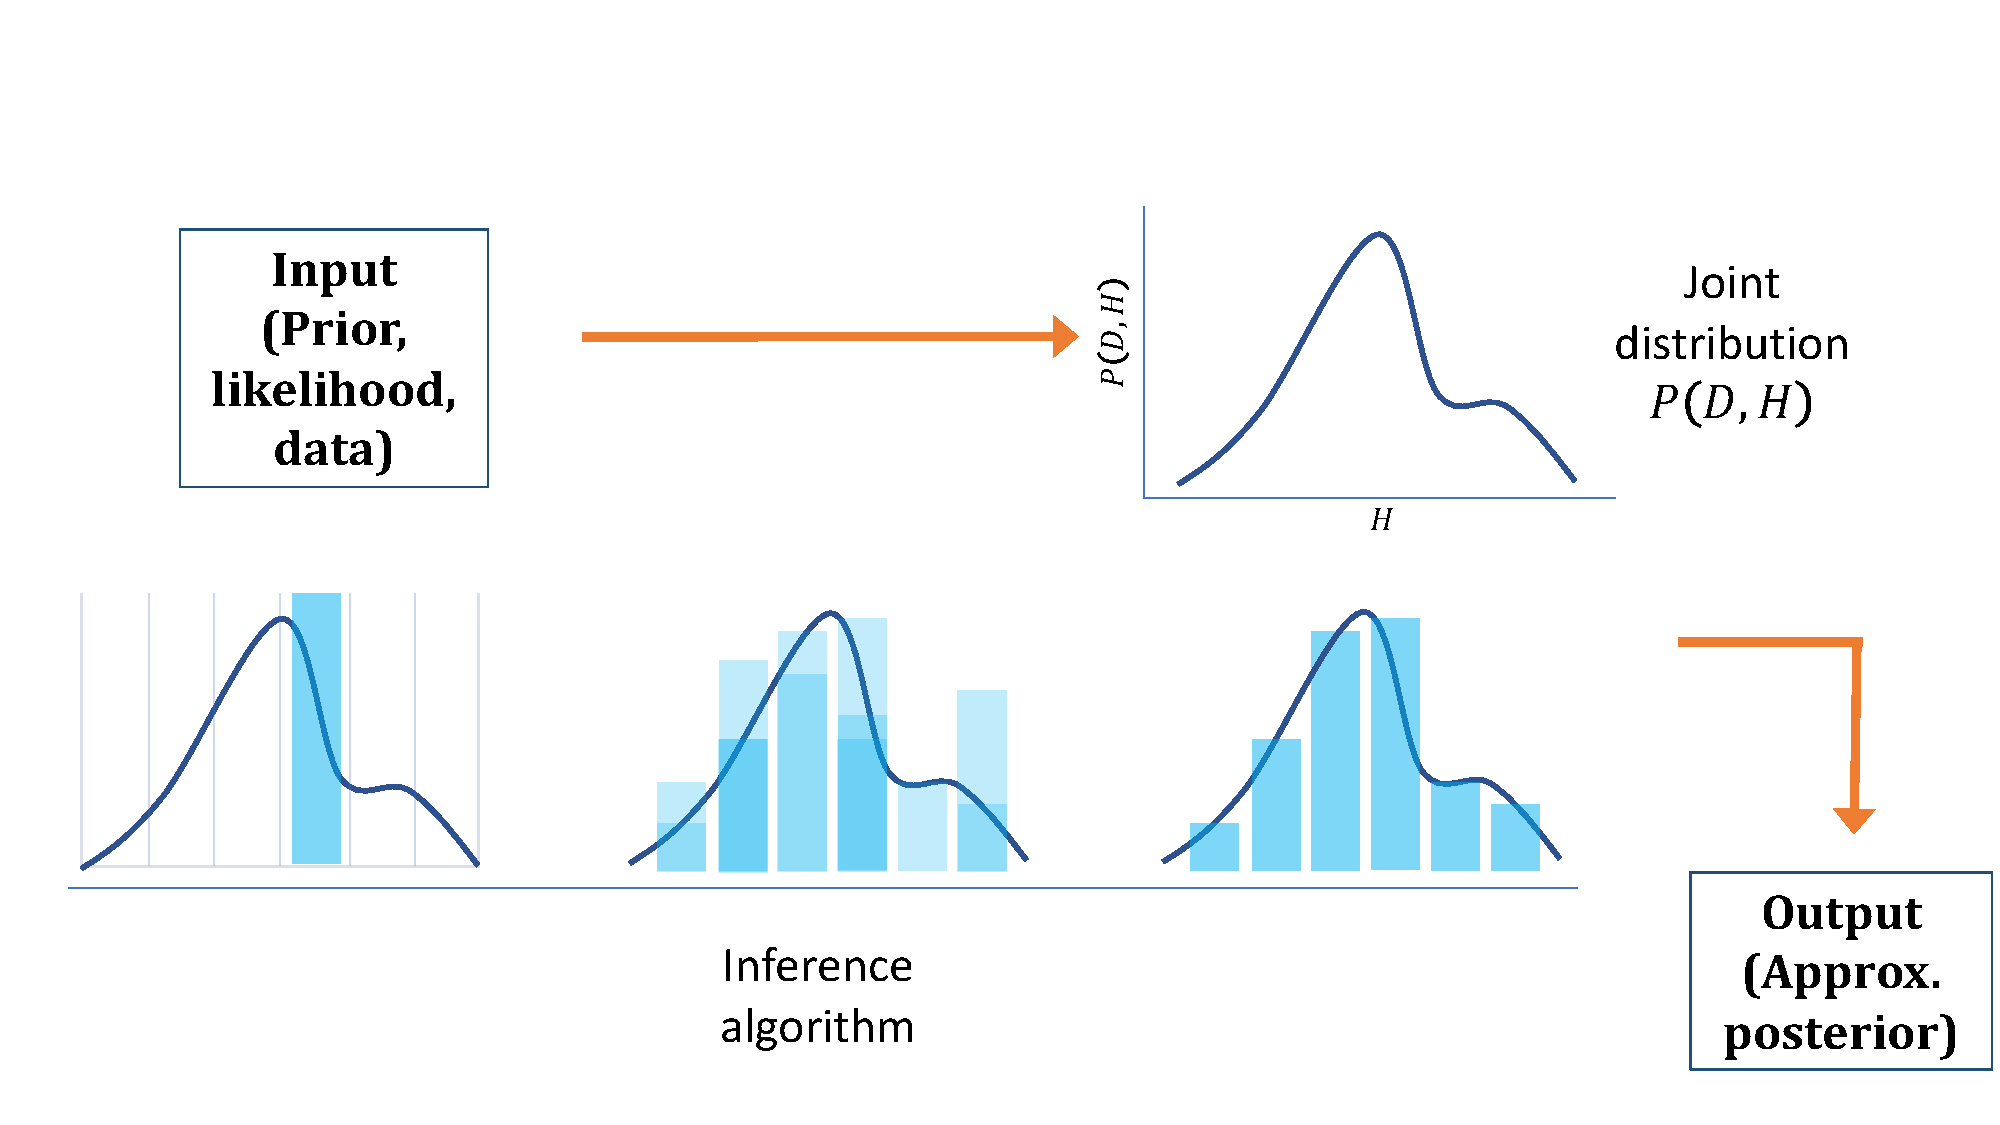
\includegraphics[width = \textwidth]{figures/MonteCarlo_schematic.pdf}
\caption{\textbf{Schematic for Monte Carlo approximation}. }
\label{fig:MC_schematic}
\end{figure}

In general, we cannot directly sample from the posterior, because the normalizing constant $P(d) = \sum_{h} P(h,d)$ requires the evaluation of the joint probabilities of each and every hypothesis and is intractable when the hypothesis space is large. In fact, sampling from the exact posterior entails solving exactly the problem which we wish to approximate. Nonetheless, it is still possible to construct an asymptotically exact approximation by sampling from a Markov chain whose stationary distribution is the posterior; this method is known as \emph{Markov chain Monte Carlo} (henceforth referred to as MCMC). \footnote{There exist other Monte Carlo methods that do not simulate a Markov chain. These include accept-reject methods and importance sampling. While these have the advantage of producing uncorrelated i.i.d. samples, they do not scale well to high dimensions, and often require pre-existing knowledge of the posterior. This makes MCMC methods the predominant Monte-Carlo method commonly used for Bayesian inference \cite{neal1993probabilistic, andrieu2003introduction}.}.

\subsection{Algorithmic details}

In this section we describe the mechanism of a specific variant of MCMC called Metropolis-Hastings. We will briefly also discuss another variant Gibbs sampling, as a specific case of Metropolis-Hastings.

We assume that the joint distribution is known. Therefore, although we cannot evaluate $P(h | d)$ at any given $h$ since we do not know the normalization factor, we can evaluate relative probabilities between the probabilities of two hypotheses very easily. We also assume a proposal distribution $Q(h)$. We will discuss teh import of the choice of this proposal distribution later in the section. 

The goal is to create samples from some probability distribution $P(h | d)$. The output therefore should be a set of different hypothesis denoted $S$ that occur with frequencies determined by $P(h | d)$. This set $S$ determines our sample based approximation $\hat{P}_N(h|d) $. Its size is determined by how many steps $N$ we run the chain for. The procedure we follow is:
\begin{itemize}
\item Start the Markov chain at any random hypothesis $h$. Add it to $S$.
\item Propose a new hypothesis $h'$ by sampling $Q$.
\item Calculate the Metropolis-Hastings acceptance probability $a = \text{min}\left( \frac{P(h' | d) Q(h))}{P(h | d) Q(h')}, \right)$
\item Flip a coin that lands Heads with probability $a$.
\item If the coin lands Heads then accept the proposal $h'$ and add it to $S$. Else reject the proposal and stay at $h$ and add it to $S$ again.
\item Repeat steps 2 onward $N$ times.
\end{itemize}

This results in a Markov chain with $P(h|d)$ as its stationary distribution, see \citet{blitzstein2014introduction} for proofs. As  $N \rightarrow \inf$, the approximation $\hat{P}_N(h|d) $ asymptotically approaches the true posterior $P(h | d)$. See Holden 1998 \cite{holden1998geometric} for proofs.

What remains to be decided is what a good proposal distribution might be. The closer the proposal to the true posterior, the faster the algorithm converges\cite{holden1998geometric}. The proposal distribution can also depend on the current state of the Markov chain, allowing for local adjustments to the current hypothesis. Another well known variant of MCMC called Gibbs sampling can be seen as a variant of Metropolis-Hastings, with a specific proposal distribution such that the proposals are always accepted. Here the sampling is over a joint distribution over hypotheses $\vec{h}$ that have multiple ($k$) dimensions. Only one of these dimensions $h_i$ is changed in every step, and the proposal distribution is the exact conditional distribution $Q = P(h_i | h_{1:K\setminus i})$. Substituting this into the formula for the acceptance probability, we can see that this proposal is always accepted. The conditional distributions however are not always easy to compute, making Metropolis-Hastings a more general purpose MCMC algorithms (though with the added worry of choosing a good proposal distribution).

\subsection{History}
Sampling methods based on Markov chains were first developed in physics to study properties of the Boltzmann distribution in statistical mechanics. \cite{metropolis1953equation} For a system at equilibrium, the relative frequency of a configuration $\omega$ is given by its Boltxmann weight

\begin{align}
e ^{-E(\omega) / kT}
\end{align}

where $T$ is the temperature and $k$ is the Boltzmann's constant. The probability distribution over configurations therefore is given by 

\begin{align}
P(\omega) = \frac{ e ^{-E(\omega) / kT}} {Z} = \frac{ e ^{-E(\omega) / kT}} {\sum_{\omega'} e ^{-E(\omega') / kT}}
\end{align}

where the denominator $Z$ is called the partition function. This partition function in reaslistic cases is computationally intractable. This has striking resemblances to the problem of Bayesian inference we described above -- where relative probabilities are easy to compute, but exact probabilities are prohibitive due to the evaulation of an intractable normlizating constant. 

The original paper \citet{metropolis1953equation} introduced the \textit{Metropolis} algorithm, where the proposal is limited to being local. It was further generalized, and formalized mathematically in \citet{hastings1970monte} to give the modern \textit{Metropolis-Hasting algorithm} decribed in the previous section.

Versions of MCMC were then applied to optimization problems in the form of \textit{simulated annealing} \cite{kirkpatrick1983optimization}, widening their reach out outside of statistical physics. The first Bayesian perspective (as well as a new MCMC algorithm, Gibbs sampling) came from an application of MCMC to the problem of digital restoration\cite{geman1984stochastic}. These methods have since been widely applied in physics, engineering, and artificial intelligence, see \citet{richey2010evolution} for further details on the history of MCMC.


\subsection{Monte Carlo methods in models of cognition}

Sampling theories have long been invoked, implicitly or explicitly, in models of human cognition to justify variation in responses across individuals and trials. In studies demonstrating optimal Bayesian behavior in the average, it has often been found that individual reponses arise from the full range of the distribution, with frequency proportional to the posterior probability, in a phenomena called `probability matching' \citep{wozny2010,Denison2013,Moreno11,Vul2014}. More recently,``rational process models'' have explicitly modelled sampling as a mechanism to drive a stronger connection between rational models of cognition and psychological mechanisms \cite{griffiths2012bridging, Vul2014, shi10, sanborn2010rational, Lieder2013}. These highlight phenomena that emerge in the finite sample regime, within a ``resource-rational'' framework \citep{Vul2014,griffiths2015,Gershman2015,schulz2016simple}. This framework posits the if generating samples is costly (in terms of time and cognitive resources), then the rational strategy is to generate the minimum number of samples necessary to achieve a desired level of accuracy. This explicitly bridges the requirements from a computational level account of inference, with the cognitive processes that implement it. 
%An important implication of this framing is that that incentives or uncertainty should have systematic effects on sample generation. For example, \citet{hamrick2015think} showed that people generated more samples when they were more uncertain. By the same token, cognitive load \citep{sprenger2011} or response time pressure \citep{Dougherty2003} act as disincentives, potentially reducing the number of generated samples.

We have so far discussed the advent of Monte Carlo approximations in cognitive science more broadly, without considering specific algorithms for it. The two main contenders have been importance sampling \cite{shi10} and MCMC \cite{Lieder2013}. In this thesis we discuss MCMC in particular for a few reasons. First, MCMC does not require knowledge of normalized probabilities at any stage and relies solely on an ability to compare the relative probabilities of two hypotheses. It has been shown in the literature \citep{stewart06} that humans have a better sense for relative rather than absolute probabilities. Second, MCMC allows for feedback between the generation and evaluation processes. The evaluated probability of already generated samples influences if and how many new samples will be generated, consistent with adaptive generation of samples like in \citet{hamrick2015think}. Third, Markov chains generate autocorrelated samples, consistent with autocorrelation in hypothesis generation \citep{multistability,vul08,Bonawitz2014}. Correlation between consecutive samples manifested as anchoring effects (where judgments are biased by the initial hypothesis \citep{tversky}) are replicated by MCMC approximations that are also transiently biased (during the``burn-in'' period) by their initial hypothesis, prior to reaching the stationary distribution \citep{Lieder2013}. Finally, work in theoretical neuroscience has shown how MCMC algorithms could be realized in generic cortical circuits \citep{buesing11,pecevski11,Moreno11}. In Chapter \ref{chap:MCMC} we discuss in greater detail the unique predictions of MCMC as compared to other sampling algorithms that have been explored in the psychological literature, like importance sampling.
%
%%% Include here?  It doesn't require knowledge of normalized probabilities at any stage and relies solely on an ability to compare the relative probabilities of two hypotheses. This is reassuring because it is much more natural to expect that humans can gauge the relative probabilities of hypotheses better than their absolute probabilities \citep{stewart06}.
%%ERIC: Just as a side note, I'm not sure if the Stewart paper is the normal reference for that. Absolute vs relative probabilities goes all the way back to Kahneman vs. Gigerenzer
%
%To highlight the distinctive predictions of MCMC, it is useful to compare it with other sampling algorithms that have been explored in the psychological literature. \emph{Importance sampling} also uses a proposal distribution $Q(h)$, but unlike MCMC it samples multiple hypotheses independently and in parallel. These samples are then weighted to obtain an approximation of the posterior:
%\begin{align}
%\hat{P}_N(h|d) = \frac{1}{N} \sum_{n=1}^N \mathbb{I}[h_n=d] w_n,
%\end{align}
%where $w_n$ is an ``importance weight'' for sample $n$ computed according to:
%\begin{align}
%w_n \propto \frac{P(h_n,d)}{Q(h_n)}.
%\end{align}
%Intuitively, the importance weight corrects for the fact that the importance sampler draws samples from the wrong distribution. \citet{shi10} have shown how this algorithm can be used to simulate human performance on a wide range of tasks. They also identified a correspondence between importance sampling and exemplar models, which have been widely applied in psychology. In related work, \citet{shi2009neural} demonstrated how importance sampling could be realized in a biologically plausible neural circuit \citep[see also][]{abbott13}.
%
%Some of the effects we have replicated in this work could also be captured by an importance sampling algorithm with limited samples. \citet{Thomas2008} have proposed a model, HyGene, that is similar in spirit to an importance sampler with limited samples, with a memory driven proposal distribution that selects the hypotheses to be generated. HyGene explains subadditivity in terms of a failure to retrieve all the relevant hypotheses from memory due to stochastic noise in the retrieval process and limited working memory capacity.
%
%The self-generation effect can to some extent be reproduced by importance sampling because prompting a hypothesis causes it to be sampled an extra time. So the probability of the focal space will be slightly larger if hypotheses in it are explicitly prompted (other-generated and presented to the participant) than if it they are generated without prompting (self-generated). However, Experiment 2 in \cite{conf} shows that in a situation where all the alternatives are specified, prompting specific hypotheses (as in the other-generated scenarios), does not result in a higher probability judgment than when these hypotheses are not prompted (as in the self-generated scenarios). The MCMC algorithm captures this finding because in a small hypothesis space, the Markov chain will visit all the hypotheses with the right frequency irrespective of initialization. By contrast, the importance sampler predicts a higher probability for other-generated hypotheses, contrary to the empirical finding.
%
%This brings us to a key difference between importance sampling and MCMC: Importance sampling generates all hypotheses in parallel---the generation of new hypotheses has no dependence on hypotheses that have already been generated. Without this dependence, there is no interaction between the generation and evaluation processes. MCMC captures this dependence by sequentially generating hypotheses. Our model's explanation of the self-generation effect, superadditivity, the weak evidence effect and the dud alternative effect rests on this dependence. The Markov chain can get `stuck' (at least temporarily) by rejecting proposals, thus generating fewer alternatives. If, on the other hand, the current hypothesis has low probability, more alternatives are generated and the probability estimate of the focal space is reduced.
%
%The important sampler does not produce these effects, because its mechanism for generating new hypotheses is independent of the probability of the current one. If anything, prompting a hypothesis within the focal space, no matter how atypical, causes it to be sampled, \textit{increasing} the importance sampler's estimate for the probability of the focal space, contradicting superadditivity.
%
%Another key difference between MCMC and importance sampling is that MCMC generates correlated samples, whereas consecutive samples from an importance sampler are totally independent. This prevents the importance sampler from reproducing the effects in Table \ref{tab:biases} that rely on correlated sampling, such as the anchoring effect and the crowd within.
%
%Importance sampling has also been adapted to inference in dynamical systems by generating hypotheses online---a technique known as \emph{particle filtering}. This approach has been fruitfully applied to a number of domains in psychology, such as multiple object tracking \citep{vul2009explaining} and change detection \citep{brown09}. Although hypotheses are generated sequentially by particle filtering, it is important to note that this structure is dictated by the sequential nature of the generative process. For example, in multiple object tracking, the object positions are dynamic latent variables; particle filtering generates new hypotheses about the positions after each new data point is observed. In contrast, the sequences of hypotheses generated by MCMC algorithms are purely mental, in the sense that hypotheses are generated sequentially regardless of whether the generative process is itself sequential. In this paper, we focus on non-sequential generative models in order to stress this point.
%
%

\section{Variational methods}

To motivate variational approximations, we first consider a more general case of Monte Carlo approximation, using weighted samples
\begin{align}
    P(h|d) \approx \sum_{n=1}^N w^n \mathbb{I}[h^n = h],
    \label{eq:montecarlo}
\end{align}
Monte Carlo algorithms can be thought of as procedures for generating an approximate posterior $Q_\phi(h|d)$ parametrized by the set of these weights and samples, $\phi = \{ w^n, h^n \}_{n=1}^N$. The superset $\Phi$ of all feasible sets (i.e., the sets that can be produced by a particular Monte Carlo algorithm) defines an approximation family. This leads us to a more general view of approximate inference as an optimization problem: find the approximation (parametrized by $\phi \in \Phi$) that gets ``closest'' to the true posterior, where dissimilarity between the two distributions is measured by a divergence functional $\mathcal{D}$. 
\begin{align}
\phi^\ast = \argmin_{\phi \in \Phi} \mathcal{D}[Q_\phi(h|d)||P(h|d)],
\end{align}
Monte Carlo algorithms do not solve this optimization problem, but instead randomly sample $\phi$ such that, in the limit $N \rightarrow \infty$, they produce $\phi^\ast$. It is however possible to design non-randomized algorithms that directly optimize $\phi$ even in a sample-based approximation\citep{saeedi2017variational}. Such optimization is an example of \emph{Variational Inference} \citep{jordan1999introduction}.

The general idea of Variational Inference (VI) is to first posit a family of densities and then to find a member of that family which is closest to the target probability distribution. Classic variational methods use the \textit{Kullback-Leibler} divergence (also known as relative entropy) as a measure of closeness. This is given by:
\begin{align}
\mathcal{D}_{\text{KL}}[Q_\phi(h|d)||P(h|d)] = \sum_h Q_\phi(h|d) \log \frac{Q_\phi(h|d)}{P(h|d)}.
\end{align}
This formulation reduces the problem of approximate inference to an optimization problem to which any standard algorothm for optimization may be applied. An example with a Gaussian approximation family and an iterative optimization procedure is given in Figure \ref{fig:var_schematic}.

In general however, this divergence cannot directly be optimized, since finding a $Q$ that optimizies $\mathcal{D}_{\text{KL}}$ requires knowing the exact $P$ -- which is precisely the problem we are trying to approximate. Instead we optimize an alternative objective that is equivalent to $\mathcal{D}_{\text{KL}}$ up to an added constant,

\begin{align}
\text{ELBO}[Q_\phi(h|d)] &=  \sum_h Q_\phi(h|d) \log \frac{P(h,d)}{Q_\phi(h|d)} \\
& = \sum_h Q_\phi(h|d) \log \frac{P(h|d)}{Q_\phi(h|d)} + \sum_h Q_\phi(h|d) \log P(d) \\
& = - \mathcal{D}_{\text{KL}}[Q_\phi(h|d)||P(h|d)]  + \log P(d)
\end{align}

This function is called the evidence lower bound, or ELBO. It is computable because the joint distribution $P(h, d)$ in known. The log probability of the observed data $P(d)$ is independent of the approximation $Q_\phi(h|d)$, so maximizing the the ELBO is equivalent to minimizing $\mathcal{D}_{\text{KL}}[Q_\phi(h|d)||P(h|d)] $.

\begin{figure}
\centering
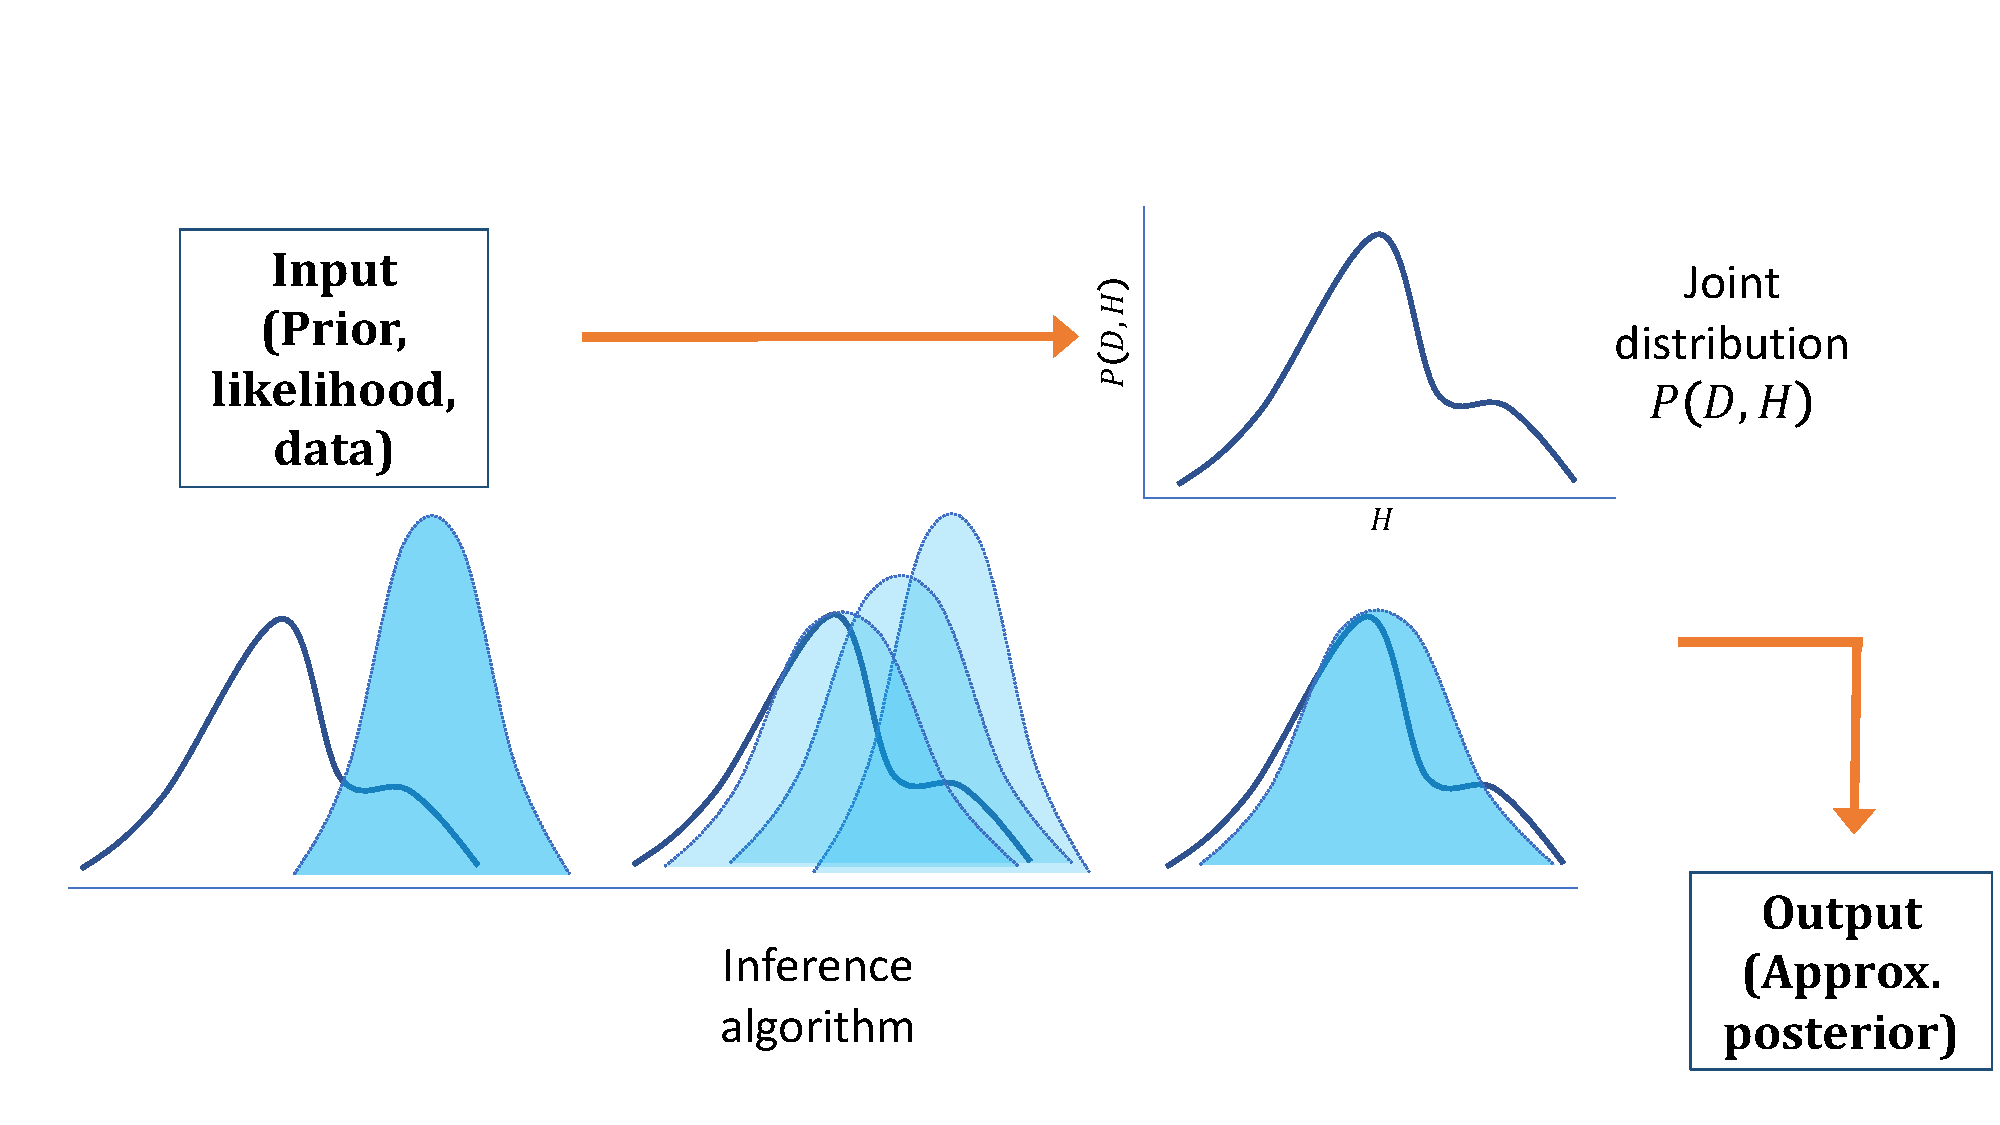
\includegraphics[width = \textwidth]{figures/variational_schematic.pdf}
\caption{\textbf{Schematic for Variational approximation}. }
\label{fig:var_schematic}
\end{figure}


\subsection{Algorithmic details}


Blackbox variational inference
In the main text, the variational optimization problem is stated in terms of minimizing KL divergence. This is useful for clarifying the nature of the problem, but less useful from an algorithmic perspective because the objective function is not tractable (it requires knowledge of the true posterior distribution, which is what we are trying to approximate). Nonetheless, we can obtain a tractable objective function using the following identity:
\begin{align}
    \log P(d) = \mathcal{L}[Q_\phi(h|d)] + \mathcal{D}_\text{KL}[Q_\phi(h|d)||P(h|d)],
\end{align}
where
\begin{align}
    \mathcal{L}[Q_\phi(h|d)] = \mathbb{E}_{Q_\phi(h)} \left[ \log P(h,d) - \log Q_\phi(h) \right]
\end{align}
is the \emph{evidence lower bound} (ELBO), also known as the \emph{negative free energy}. The term ELBO comes from the fact that $\mathcal{L}[Q_\phi(h|d)]$ is a lower bound on the ``evidence'' (log marginal likelihood) $\log P(d)$. Maximizing the ELBO will produce the same variational approximation as minimizing the KL divergence. Critically, the ELBO eliminates the dependence on $P(h|d)$, only requiring access to the unnormalized posterior, the joint distribution $P(h,d)$.

In certain special cases, the ELBO can be tractably computed \citep[see][]{jordan1999introduction}, but this is not true for arbitrary joint distributions and approximations. Because the Learned Inference Model uses a flexible neural network function approximator, we adopt an approximate technique for evaluating and optimizing the ELBO known as \emph{blackbox variational inference} \citep{ranganath2014black}. The key idea is to approximate the gradient of the ELBO with a set of $M$ samples:
\begin{align}
    \nabla_\phi \mathcal{L}[Q_\phi(h|d)] \approx \frac{1}{M} \sum_{m=1}^M \nabla_\phi \log Q_\phi(h^m|d) \left[ \log P(h^m,d) - \log Q_\phi(h^m) \right],
\end{align}
where $h^m \sim Q_\phi(h|d)$. Using this approximation, the variational parameters can be optimized with stochastic gradient descent updates of the form:
\begin{align}
    \phi_{t+1} \leftarrow \phi_t + \rho_t \nabla_\phi \mathcal{L}[Q_\phi(h|d)],
\end{align}
where $t$ indexes iterations and $\rho_t$ is an iteration-dependent step-size. Provided $\rho_t$ satisfies the Robbins-Monro stochastic approximation conditions ($\sum_{t=1}^\infty \rho_t = \infty, \sum_{t=1}^\infty \rho_t^2 < \infty$), this optimization procedure will converge to the optimal parameters with probability 1.
\subsection{History}

The history of variational inference is more difficult to trace since it is intimately tied to optimization. Some of the first variational approximations appear in statistical physics as mean field theories. The first of these was the Curie-Weiss theory for ferromagnetism, that made a mean-field approximation to the Ising model\cite{curie1895proprietes,  weiss1907hypothese}. Here the local field at each point on a lattice, which could in theory have significant local structure, is approximated by a global field that applies uniformly to the whole lattice. This effectively ignores correlations between the lattice sites. In the language of the previous section, this constitutes approximating the probability distribution $P(\vec{h})$ which maybe be defined over a complex joint distribution over the dimensions of $\vec{h}$. 

Subsequent to this model, several other mean field theories were developed across other domain of physics. \citet{landau1965collected} formalized mean field theory as a variational approximation\cite{kadanoff2009more}. Concurrently, variational approaches were also applied to problems in quantum physics and quantum field theory \citep{milton2006electromagnetic, feynman1965quantum}. 

The development of variational methods specifically for Bayesian inference is relatively more recent, arguably starting with a mean field learning algorithm for neural networks in \citet{anderson1987mean}, followed by formalization of variational approximations to a slew of othe models\citep{saul1996mean, jaakkola1997variational}. These approaches have been extensively studied in statistics and machine learning, and provide a strong alternative to MCMC for scalable posterior approximation \citep{blei2017variational}.

\subsection{Variational methods in models of cognition}

The variational optimization view of approximate inference allows us to consider more general approximation families that go beyond weighted samples. In fact, the approximate posterior can be any parametrized function that defines a valid probability distribution over the relevant hypothesis space. For example, researchers have used deep neural networks as flexible function approximators \citep{dayan1995helmholtz,kingma2014auto,mnih2014neural,rezende2015variational,paige2016inference}. From a neuroscience perspective, this approach to approximate inference is appealing because it lets us contemplate complex, biologically realistic approximation architectures \citep[provided that the optimization procedures can also be realized biologically; see][]{whittington2019theories}. For example, particular implementations of variational inference have been used to model hierarchical predictive coding in the brain \citep{friston2008hierarchical,gershman2019does}.


\section{Hybrid methods}

